% Design of Algorithms (1 week)

\deff{Algorithm}{An algorithm is a well-defined computational procedure with input values and output values.}

In order to be able to compare different algorithms, they are compared in terms of their efficiency. For the \emph{computational time}, the proportionality relationship between the \emph{running time} (number of primitive operations) and the input size $N$ is decisive. A simplified parameter is the order of growth $\Theta$ (e.g. $\Theta(N^2)$ or $\Theta(\log N)$), which describes how the running time scales with the input size $N$. For each algorithm, it is possible to determine what the running time is in the best case (lower bound) and in the worst case (upper bound).

\subsection{Brute Force}

\deff{Brute Force}{Brute force refers to an algorithm that solves the problem exclusively in a linear fashion, which is usually very inefficient.}

The brute force algorithm to sort a vector of integers is the \emph{Selectionsort} algorithm. In this algorithm, a vector $a$ is sorted by checking for each vector element $i$ (outer loop) individually whether there is a smaller element $j$ in the remaining vector (inner loop) and, if so, swapping the smallest element found with the element under consideration. The vector is then sorted from left to right. As the vector is passed through twice, the algorithm with $\Theta(N^2)$ is relatively inefficient.

\begin{center}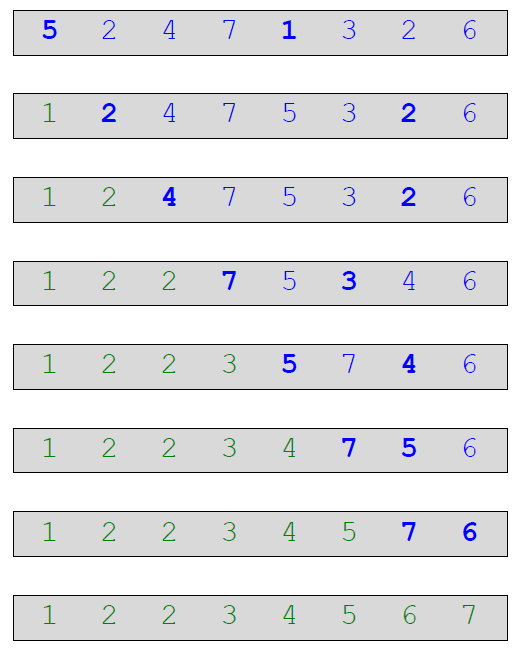
\includegraphics[width=0.85\textwidth]{img/algorithms/BruteForceSelectionsort.png}\end{center}

%\lstinputlisting[language=C++]{src/algorithms/selectionsort.cpp}

\subsection{Divide-and-conquer}

\deff{Divide-and-Conquer}{The divide-and-conquer is a recursive algorithm that consists of dividing the problem into simpler subproblems, solving these individually and finally combining the individual solutions into an overall solution.}
\begin{enumerate}
    \item \textbf{Divide} the problem into a number of smaller subproblems that are smaller instances of the same problem.
    \item \textbf{Conquer} the subproblems by solving them recursively (if the subproblem size is small enough, solve it in a straightforward manner).
    \item \textbf{Combine/Merge} the solutions to the subproblems into the solution for the original problem.
\end{enumerate}

The algorithm is often quite efficient with $\Theta(N\log N)$. A typical example of a divide-and-conquer algorithm is the recursive sorting algorithm \emph{Mergesort}. A vector $a$ is divided into smaller vectors $b$ until the sub-vectors only contain one number. These are then combined to form the sorted vector.

\begin{center}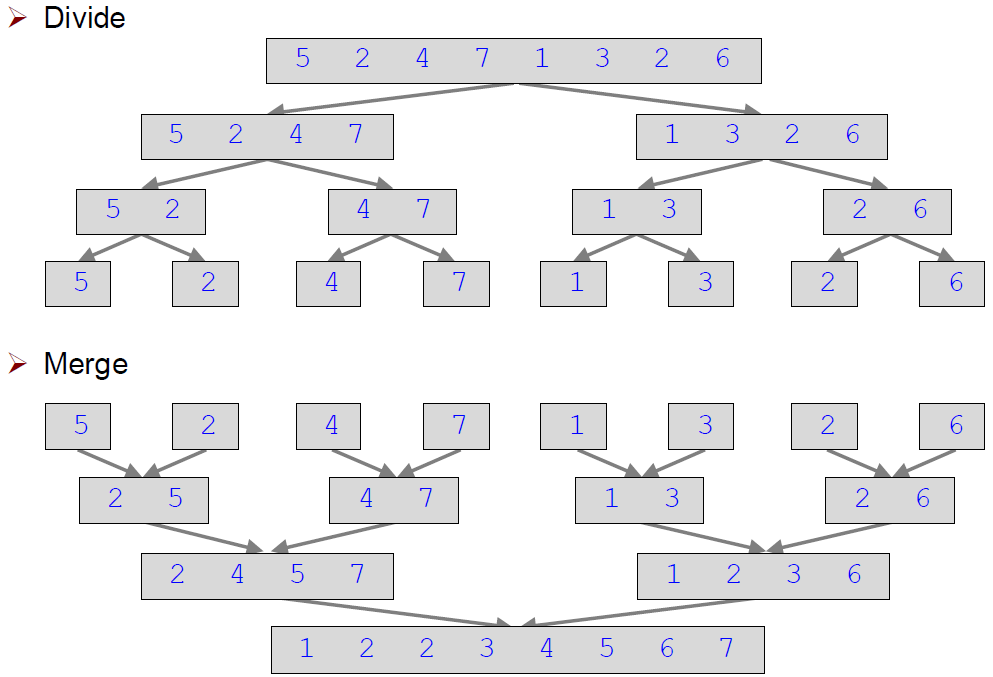
\includegraphics[width=0.85\textwidth]{img/algorithms/DivideConquerMergesort.png}\end{center}

%\lstinputlisting[language=C++]{src/algorithms/mergesort.cpp}

\subsection{Dynamic Programming}



%\lstinputlisting[language=C++]{src/algorithms/knappsack.cpp}

\subsection{Greedy Algorithm}

%\lstinputlisting[language=C++]{src/algorithms/knappsack.cpp}

\subsection{Backtracking}

%\lstinputlisting[language=C++]{src/algorithms/greedy_knappsack.cpp}

\subsection{Local Search}

%\lstinputlisting[language=C++]{src/algorithms/add_queen.cpp}